\section{Introduction}
\label{sec-introduction}

Two trends are combining to create increasingly crowded and uncoordinated
home \wifi{} environments. First, increasing broadband penetration is
creating larger numbers of private home access points (APs). Strategy
Analytics estimated that by the end of 2014, 451~M households worldwide
(25\%) would have home \wifi{} and that this number will continue to
grow~\cite{wifi-survey}. Second, an increasing percentage of the world's
population resides in dense urban environments: 54\% today and climbing to
66\% by 2050~\cite{urbanization-survey}. Together these two trends create a
future where more people will operate private home APs that overlap with
other nearby private home APs.

\begin{figure}[t]
  %
  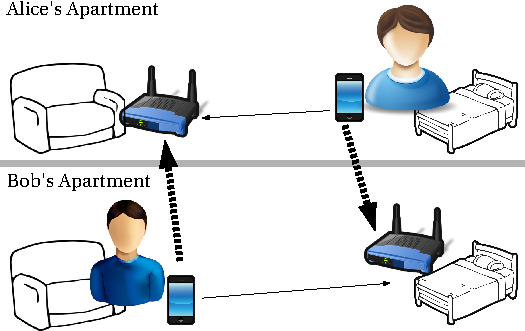
\includegraphics[width=\columnwidth]{./figures/motivation.pdf}
  %
  \caption{\textbf{Example of Reciprocal \wifi{} Sharing.} Solid arrows
  represent weak connections, while dashed lines represent strong
  connections.}
  %
  \label{fig:motivation}
  %
\end{figure}

Unfortunately, uncoordinated deployment of overlapping private networks can
create interference that degrades performance, which may then cause users to
respond in ways that further exacerbate the problem. Consider Alice and Bob's
neighboring apartments shown in Figure~\ref{fig:motivation}. Alice has
deployed her AP in her living room, while Bob has deployed his in his
bedroom. Due to the proximity of their apartments, Alice receives a stronger
signal from Bob's router when she is in her bedroom. But because she cannot
connect to Bob's router, she must either use the lower-bandwidth connection
to her existing AP or deploy an additional AP in her bedroom. Both of these
options generate additional wireless interference for her neighbors,
including Bob. And while we have used Alice as an example, Bob also faces the
same poor choice.

However, due to factors such as blockage or fading in wireless signal
propagation, home \wifi{} AP usually does not provide equally satisfying \wifi{}
coverage at all places within the house. Instead, it is likely that the user
receives better \wifi{} signal from a neighbor's AP at certain spots. For
instance, consider Alice and Bob who live in neighbor apartments, as shown in
Figure~\ref{fig:motivation}, each of them receives a stronger \wifi{} signal
from the other's home AP than their own at certain places within their
apartments, revealing a \textit{reciprocal} \wifi{} sharing opportunity where
both parties can improve their \wifi{} performance by allowing each other to
access their own private networks.

Compared to traditional community networks such as FON~\cite{fon} or
OpenWireless~\cite{openwireless}, such reciprocal sharing opportunity has
several unique properties that make it interesting to explore. First, such
opportunity is usually \textit{immediate} between two physically colocated
parties, such as two neighbors. This helps relief the concerns of sharing
network to random strangers in traditional community networks and makes it more
practical to establish the sharing. Second, bonding to physical colocation
relationship makes the opportunity \textit{stable} over time, enabling
asynchronous fair sharing over longer period of time.


Nevertheless, there are several challenges in fulfilling the vision of
reciprocal \wifi{} sharing shown in Figure~\ref{fig:motivation}. First, although
the motivating example is inspired by the authors' own experience, it is not
clear how often such opportunity exists for broader range of users in real life
scenarios. Second, suppose the sharing opportunity does exist and is detected,
there is no systematic solutions to enable the \wifi{} sharing without
compromising the security and privacy of user's home network. Finally, after the
\wifi{} sharing is established, it is challenging to ensure that the
relationship remains reciprocal for both parties.

To address these challenges, we first present extensive analysis of the
\PhoneLab{} \wifi{} dataset which contains \num{21192417} scan results from 254
smartphones over 5 months (Section~\ref{sec:investigation}). The results show
that such reciprocal \wifi{} sharing opportunities does exists even in a spatial
sparse dataset. Inspired by the results, we present the design of \wisefi{}
(Section~\ref{sec:design}), a system that detects such reciprocal \wifi{}
sharing opportunities using smartphones, enables \wifi{} sharing on APs with or
without guest network support, and ensures the sharing remain reciprocal.
Finally, we discuss some open challenges in implementing such a system and point
directions for future works (Section~\ref{sec:challenges}).
